\documentclass[../../main]{subfiles}

\renewcommand\thesection{\arabic{section}}


\begin{document}

\section{12V to Lower Voltages} \label{sec:}

Now that we have 12V supply, we need to convert this to lower voltages.
For everything expect, the \emph{sensors}, \emph{relays}, \emph{peltier},
and \emph{fans} uses 5V. \emph{Sensors} use 3.3V and the others mentioned
above uses 12V itself. So we need to generate the 5V and 3.3V for all the
other components.

For 5V, we can use \emph{LM2596}, which is DC-DC buck converter. We will be
using total of 3 of these to generate 5V. Refer figure \ref{fig:buckConverterImage}
for a quick glance at the device.

\begin{center}
    {\begin{minipage} [c] {0.55\textwidth}

        Specification:

        \begin{itemize}
            \item \textbf{Input voltage:} $3.2 \si{V}$ to $40 \si{V}$.
            \item \textbf{Output voltage:} $1.25 \si{V}$ to $35 \si{V}$.
            \item \textbf{Output current:} $2 \si{A}$.
            \item \textbf{Output current max.:} $3 \si{A}$.
        \end{itemize}

    \end{minipage}
    \hfill
    \begin{minipage} [c] {0.35\textwidth}
        \centering
        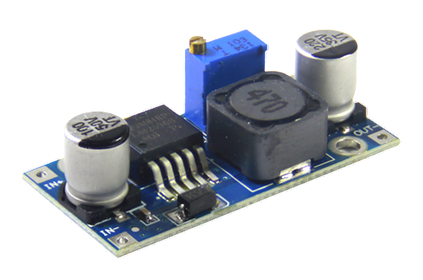
\includegraphics [
            max width = \IGXMaxWidth,
            max height = \IGXMaxHeight,
            \IGXDefaultOptionalArgs,
        ] {pics/buck_converter.png}
        \captionof{figure} {
            \emph{LM2596}.
            \label{fig:buckConverterImage}
        }
    \end{minipage}\hfill}
\end{center}

\alertNote{
    The 3.3V power supply for the sensors are taken from the \texttt{3V3} pin of \esp.
}

\end{document}
